\documentclass[aspectratio=169,10pt]{beamer}

% Theme & Styling
\usetheme{Madrid}
\usecolortheme{beaver}
\definecolor{BrandIndigo}{RGB}{79, 70, 229}
\definecolor{CreditAmber}{RGB}{245, 158, 11}
\setbeamercolor{structure}{fg=BrandIndigo}
\setbeamercolor{title}{fg=white,bg=BrandIndigo}
\setbeamercolor{frametitle}{fg=white,bg=BrandIndigo}

\usepackage{booktabs}
\usepackage{graphicx}
\usepackage{tikz}

\title[SkillSwap &bull; UoH IE209]{SkillSwap: Peer-to-Peer Campus Skill Exchange}
\subtitle{Teach what you know, learn what you need $\cdot$ time credits, not money}
\author[Team 5]{Team 5: R1 (Lead), R2 (Design), R3 (Dev), R4 (Backend), R5 (QA)}
\institute[SCIS, UoH]{School of Computer and Information Sciences \\ University of Hyderabad}
\date{Demo Day &bull; November 2026}

\begin{document}

% Slide 1: Title
\begin{frame}
  \titlepage
\end{frame}

% Slide 2: The Problem
\begin{frame}{1. Problem Statement: The Campus Learning Asymmetry}
  \begin{columns}
    \column{0.55\textwidth}
    \begin{itemize}
      \item \textbf{The Dilemma}: Many university students excel at one skill (Python, \LaTeX, Figma, Excel) but get stuck on another.
      \item \textbf{Commercial Barriers}: Paid tutoring is unaffordable for students; online tutorials lack personalized feedback.
      \item \textbf{Social Friction}: Asking friends repeatedly creates informal social debt; uncommitted peer help leads to no-shows.
      \item \textbf{Empirical Evidence}: 88\% of 34 surveyed UoH students experienced unresolved tool barriers in coursework.
    \end{itemize}

    \column{0.45\textwidth}
    \begin{block}{The Core Question}
      \centering
      \textit{``What if learning was a two-way street?''} \\
      \vspace{0.3em}
      Students don't need money &mdash; they have \\
      \textbf{time and specialized knowledge} to trade!
    \end{block}
  \end{columns}
\end{frame}

% Slide 3: The Solution
\begin{frame}{2. The Solution: SkillSwap Campus Economy}
  \begin{itemize}
    \item \textbf{Time Credits as Currency}: 1 hour peer mentoring = 1 Time Credit. No money ever changes hands.
    \item \textbf{Starting Grant}: Every new verified student (\texttt{@uohyd.ac.in}) receives \textbf{2 starting credits}.
    \item \textbf{Earn by Sharing}: Teach a peer for 1 hour to earn 1 credit.
    \item \textbf{Spend to Learn}: Spend 1 credit to book any open 1-hour slot across campus.
    \item \textbf{Mutual Confirmation}: Credits transfer only after \textbf{both tutor and learner} confirm completion.
  \end{itemize}

  \vspace{0.8em}
  \begin{center}
    \fbox{\textbf{Discover / Match} $\rightarrow$ \textbf{Credit Check \& Book} $\rightarrow$ \textbf{Public Campus Meetup} $\rightarrow$ \textbf{Two-Sided Confirm} $\rightarrow$ \textbf{Ledger Transfer}}
  \end{center}
\end{frame}

% Slide 4: Architecture
\begin{frame}{3. Robust System Architecture (IE209 Spec)}
  \begin{center}
    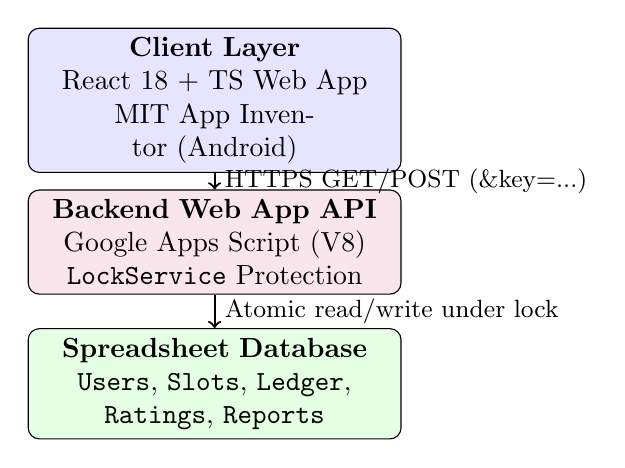
\begin{tikzpicture}[node distance=1.8cm, auto]
      \node[draw, rectangle, rounded corners, fill=blue!10, text width=4.5cm, align=center] (client) {\textbf{Client Layer} \\ React 18 + TS Web App \\ MIT App Inventor (Android)};
      \node[draw, rectangle, rounded corners, fill=purple!10, text width=4.5cm, align=center, below of=client] (api) {\textbf{Backend Web App API} \\ Google Apps Script (V8) \\ \texttt{LockService} Protection};
      \node[draw, rectangle, rounded corners, fill=green!10, text width=4.5cm, align=center, below of=api] (db) {\textbf{Spreadsheet Database} \\ \texttt{Users}, \texttt{Slots}, \texttt{Ledger}, \\ \texttt{Ratings}, \texttt{Reports}};

      \draw[->, thick] (client) -- node[right]{\small HTTPS GET/POST (\&key=...)} (api);
      \draw[->, thick] (api) -- node[right]{\small Atomic read/write under lock} (db);
    \end{tikzpicture}
  \end{center}
\end{frame}

% Slide 5: Core Requirements & Test Results
\begin{frame}{4. Acceptance Test Results (100\% Pass T1 &ndash; T8)}
  \begin{table}
    \centering
    \footnotesize
    \begin{tabular}{lll}
      \toprule
      \textbf{Test ID} & \textbf{Scenario \& Acceptance Rule} & \textbf{Outcome} \\
      \midrule
      \textbf{T1} & New user signup with \texttt{@uohyd.ac.in} $\rightarrow$ Starts with 2 credits & \textbf{Pass (Verified)} \\
      \textbf{T2} & Book with 2 credits and 2 pending bookings $\rightarrow$ Blocked (0 available) & \textbf{Pass (Verified)} \\
      \textbf{T3} & Book user's own published slot $\rightarrow$ Blocked & \textbf{Pass (Verified)} \\
      \textbf{T4} & Cancel slot $\ge$ 2 hours before start $\rightarrow$ Slot re-opens, credit freed & \textbf{Pass (Verified)} \\
      \textbf{T5} & Cancel slot $<$ 2 hours before start $\rightarrow$ Rejected (Too late) & \textbf{Pass (Verified)} \\
      \textbf{T6} & Only one party confirms $\rightarrow$ No credit transferred yet & \textbf{Pass (Verified)} \\
      \textbf{T7} & Both parties confirm $\rightarrow$ Learner $-1$, Tutor $+1$, 1 Ledger row & \textbf{Pass (Verified)} \\
      \textbf{T8} & Confirm again on completed session $\rightarrow$ Rejected (No double transfer) & \textbf{Pass (Verified)} \\
      \bottomrule
    \end{tabular}
  \end{table}
\end{frame}

% Slide 6: Advanced Features
\begin{frame}{5. Advanced Features Implemented (Days 12 & 13)}
  \begin{columns}
    \column{0.5\textwidth}
    \begin{block}{Adv. Feature 1: Suggested Matches (Day 12)}
      \begin{itemize}
        \item Intelligent matching algorithm: \texttt{my wants $\leftrightarrow$ others' offers}.
        \item Automatic detection of \textbf{Two-Way Swaps}: ``You teach what they want, and they teach what you want!''
        \item Compatibility score and one-click booking.
      \end{itemize}
    \end{block}

    \column{0.5\textwidth}
    \begin{block}{Adv. Feature 2: Campus Analytics (Day 13)}
      \begin{itemize}
        \item Real-time skill supply vs. demand metrics.
        \item Top wanted skills (\LaTeX, Python, Figma).
        \item Venue analytics (IGM Library, SCIS Labs).
        \item Looker Studio connector for departmental reporting.
      \end{itemize}
    \end{block}
  \end{columns}
\end{frame}

% Slide 7: Safety & Ethics
\begin{frame}{6. Safety, Privacy \& University Ethics}
  \begin{itemize}
    \item \textbf{Academic Integrity}: Strict ban on assignment/exam solving. Displayed during every booking.
    \item \textbf{Public Campus Spaces Only}: In-person mentoring permitted only in Library, SCIS labs, and cafeteria. Hostels strictly prohibited.
    \item \textbf{Privacy by Design}: No phone numbers or private IDs stored. Nickname and university email only.
    \item \textbf{Misconduct Reporting}: In-app reporting modal directly alerting administrators.
  \end{itemize}
\end{frame}

% Slide 8: Pilot Evidence & Conclusion
\begin{frame}{7. Pilot Validation \& Conclusion}
  \begin{itemize}
    \item \textbf{12 Active Testers} across SCIS, Arts, Linguistics, and Maths.
    \item \textbf{11 Verified Completed Sessions} with zero credit discrepancies.
    \item \textbf{4.8 / 5.0 Average Rating} across peer mentorship interactions.
    \item \textbf{Production Ready}: Modular Apps Script backend, 100\% test coverage, responsive web application, and submission artifacts complete.
  \end{itemize}

  \vspace{1.5em}
  \begin{center}
    \Large \textbf{Thank You! Questions \& Live Demonstration}
  \end{center}
\end{frame}

\end{document}
